%%%%%%%%%%%%%%%%%%%%%%%%%%%%%%%%%%%%%%%%%%%%%%%%%%%%%%%%%%%%%%%%%%%%%%%%
%    INSTITUTE OF PHYSICS PUBLISHING                                   %
%                                                                      %
%   `Preparing an article for publication in an Institute of Physics   %
%    Publishing journal using LaTeX'                                   %
%                                                                      %
%    LaTeX source code `ioplau2e.tex' used to generate `author         %
%    guidelines', the documentation explaining and demonstrating use   %
%    of the Institute of Physics Publishing LaTeX preprint files       %
%    `iopart.cls, iopart12.clo and iopart10.clo'.                      %
%                                                                      %
%    `ioplau2e.tex' itself uses LaTeX with `iopart.cls'                %
%                                                                      %
%%%%%%%%%%%%%%%%%%%%%%%%%%%%%%%%%%
%
%
% First we have a character check
%
% ! exclamation mark    " double quote  
% # hash                ` opening quote (grave)
% & ampersand           ' closing quote (acute)
% $ dollar              % percent       
% ( open parenthesis    ) close paren.  
% - hyphen              = equals sign
% | vertical bar        ~ tilde         
% @ at sign             _ underscore
% { open curly brace    } close curly   
% [ open square         ] close square bracket
% + plus sign           ; semi-colon    
% * asterisk            : colon
% < open angle bracket  > close angle   
% , comma               . full stop
% ? question mark       / forward slash 
% \ backslash           ^ circumflex
%
% ABCDEFGHIJKLMNOPQRSTUVWXYZ 
% abcdefghijklmnopqrstuvwxyz 
% 1234567890
%
%%%%%%%%%%%%%%%%%%%%%%%%%%%%%%%%%%%%%%%%%%%%%%%%%%%%%%%%%%%%%%%%%%%
%

%AIP Reprint Class%%%%%%%%%%%%%%%%%%%%%%%%%%%%%%%%%%%%%%%%%%%%%%%%%%%%%%%%%%%%%%%%%%%%%%%%%%%%%
\documentclass[aip,prl,amsmath,amssymb,reprint,superscriptaddress]{revtex4-1} %preprint version
\usepackage{graphicx}% Include figure files
\usepackage{dcolumn}% Align table columns on decimal point
\usepackage{bm}% bold math
\usepackage{epstopdf}

    \renewcommand{\topfraction}{0.9}    % max fraction of floats at top
    \renewcommand{\bottomfraction}{0.8}    % max fraction of floats at bottom
    \setcounter{topnumber}{2}
    \setcounter{bottomnumber}{2}
    \setcounter{totalnumber}{4}     % 2 may work better
    \setcounter{dbltopnumber}{2}    % for 2-column pages
    \renewcommand{\dbltopfraction}{0.9}    % fit big float above 2-col. text
    \renewcommand{\textfraction}{0.07}    % allow minimal text w. figs
    \renewcommand{\floatpagefraction}{0.7}    % require fuller float pages
    \renewcommand{\dblfloatpagefraction}{0.7}    % require fuller float pages
    \setlength{\abovecaptionskip}{5pt}
    \setlength{\belowcaptionskip}{5pt}
    \setlength{\parskip}{0pt}
    \setlength{\textfloatsep}{5pt} 

%%%%%%%%%%%%%%%%%%%%%%%%%%%%%%%%%%%%%%%%%%%%%%%%%%%%%%%%%%%%%%%%%%%%%%%%%%%%%%%%%%%%%%%%%%%%%%%%%%

%IOP preprint class %%%%%%%%%%%%%%%%%%%%%%%%%%%%%%%%%%%%%%%%%%%%%%%%%%%%%%%%%%%%%%%%%%%%%%%%%%%%%%
%\documentclass[12pt]{iopart}
%\newcommand{\gguide}{{\it Preparing graphics for IOP journals}}
%Uncomment next line if AMS fonts required
%\usepackage{iopams}
%\usepackage{graphicx}
%\usepackage{epstopdf}  
%%%%%%%%%%%%%%%%%%%%%%%%%%%%%%%%%%%%%%%%%%%%%%%%%%%%%%%%%%%%%%%%%%%%%%%%%%%%%%%%%%%%%%%%%%%%%%%%%%
%Slava's inserts %%%%%%%%%%%%%%%%%%%%%%%%%%%%%%%%%%%%%%%%%%%%%%%%%%%%%%%%%%%%%%%%%%%%%%%%%%%%%%
%\usepackage{amsfonts}
%\usepackage{amssymb}

%\newcommand{\ptt}[1]{\frac{\partial#1}{\partial t}}
%\newcommand{\vvec}{\mathbf{v}}
%\newcommand{\Bvec}{\mathbf{B}}
%\newcommand{\Evec}{\mathbf{E}}
%\newcommand{\Jvec}{\mathbf{J}}
%\newcommand{\Avec}{\mathbf{A}}
%%%%%%%%%%%%%%%%%%%%%%%%%%%%%%%%%%%%%%%%%%%%%%%%%%%%%%%%%%%%%%%%%%%%%%%%%%%%%%%%%%%%%%%%%%%%%%%%%%

\begin{document}
\title{Variance Anisotropy in a laboratory plasma}

\author{D.A. Schaffner}
\affiliation{Swarthmore College, Swarthmore, PA, USA}
\author{M.R. Brown}
\affiliation{Swarthmore College, Swarthmore, PA, USA}
\author{V.S. Lukin}
\affiliation{Space Science Division, Naval Research Laboratory, Washington, DC, USA}

\date{\today}
\begin{abstract}
Variance anisotropy observed in magnetic fluctuations on the Swarthmore Spheromak Experiment (SSX).
\end{abstract}

\maketitle

\section{Introduction}

The solar wind turbulence community has seen a flurry of results in recent years, as diagnostic capabilities on spacecraft have steadily improved, especially in the temporal resolution which has allowed for investigation into ion, sub-ion and electron scale turbulence measurements. In addition, newer analysis techniques have been developed to better tap the details of the rich turbulent environment that is the heliosphere. 

Theoretical treatments of magnetized plasma turbulence have almost universally predicted anisotropy to develop based on directions perpendicular and parallel to a mean field vector; many forms of this anisotropy has been predicted and observed (a good overview of the various types is given in Horbury 2012)~\cite{horbury12}. This paper focuses on variance anisotropy---the observation of greater magnetic fluctuation power in components perpendicular to the mean magnetic field versus parallel. From the experimentalist point of view, this is the most straightforward quantity to report and a reasonable place to begin. Analysis of other forms of anisotropy are saved for future work.---%has garnered great interest as it is viewed as a keystone result for theoretical understanding of MHD turbulence. 

Anisotropy is a common theme in solar wind turbulence and is predicted to be present by many turbulence theories. Since the solar wind speeds are typically super-Alfvenic, anisotropy studies generally reference the velocity vector of the bulk flow when defining perpendicular versus parallel fluctuations. Variance anisotropy, however, references a mean magnetic field vector---either global or local mean.

As results from space become more detailed, comparison to simulation and laboratory experiment become more useful in order to better develop the theory as well as inform future space missions. Much progress has been made to develop laboratory experiment which can inform space plasma research~\cite{howes12a} as well as begin to make turbulence measurements~\cite{ren11}.  Experiments conducted in the MHD wind-tunnel configuration of the Swarthmore Spheromak Experiment have shown the ability to produce and analyze MHD turbulence using many of the same methods used in the space plasma community, and has produced turbulence measurements which are comparable to \textit{in-situ} results~\cite{schaffner14a}. Moreover, using varying amounts of helicity injection, some characteristics of the turbulence can be modified~\cite{schaffner14b}.

A full spectral analysis of fluctuations in the SSX has been conducted, including magnetic field, density and Mach flow fluctuations. Using a wavelet transform method to decompose the timeseries signal, the magnetic field fluctuation spectra can be broken into portions that are parallel or perpendicular to the local magnetic field vector. Analysis of these portions show that parallel fluctuation power decreases slightly faster than that for perpendicular fluctuations generating a separating in power as a function of increasing frequency. This effect in frequency space is very close to the observation of variance anisotropy seen in wavenumber space in solar wind turbulence. The ratio is shown to grow from nearly isotropic levels in the energy injection scale to a maximum $\perp/\parallel$ ratio of 3 at frequencies of about 1MHz. Beyond this point, the ratio begins to contract reaching isotropy around 10MHz. Though the axial flow speeds of the plasma in the wind-tunnel sub-Mach, if a Taylor hypthesis were still invoked this peak in the ratio would correspond to the ion inertial scale length. Comparison between magnetic flucutation spectra and flow fluctuation spectra are also reported.

The organization of this paper is as follows: First, a brief description of the plasma laboratory is given. Then, an overview of the analysis techniques used to determine perpendicular and parallel fluctuations is provided; details of the method and a second method used to verify its validity are described in the appendix. The results of this analysis is provided in section 4 including how spectra scaling varies with helicity injection, and how it evolves in time. In section 5 a comparison of magnetic fluctuation spectra is made to velocity and density fluctuations as well. Section 6 gives a discussion of how all of these spectra results are consistent with the observation of an ion inertial scale in the plasma. Comparison to a MHD simulation is made in section 7 and conclusions are presented in section 8.

\section{Experiment}

The results center around three groupings of experimental parameters of 40 shots each enumerated by a stuffing flux value. The main run has a stuffing flux value of 1.0mWb. It has average field values of 5kG and average bulk flow of M=0.6. A second run has a value of 0.5mWb, and had average field values of 5kG, but a Mach number of only 0.2. A third run has zero stuffing flux, low field values, and flows of M=0.2.

\section{Analysis Techniques}

\section{Variance Anisotropy}\label{sec:variance}

The magnetic field fluctuation spectra perpendicular and parallel to the local magnetic field vector is shown in figure~\cite{fig:spectra}(a) averaged over 40 shots and the inner four probe tips. Like previously reported magnetic spectra~\cite{schaffner14}, both perpendicular and parallel curves exhibit power-law like behavior for most frequencies between 10kHz and 10MHz. Fits can be made to various sections of the curve using a Maximum Likelihood Estimation method~\cite{clauset09}; the short fits show that the scaling appears to gradually change from spectral indices of about 1 in the injection (or outer) range and from about 2.5 to 5 in the remaining sections. As has been noted before, with the exception of the injection range slope, the inertial and possibly dissipation range spectral indices are steeper than observed in solar wind turbulence spectra.

\begin{figure}[!htbp]
\centerline{
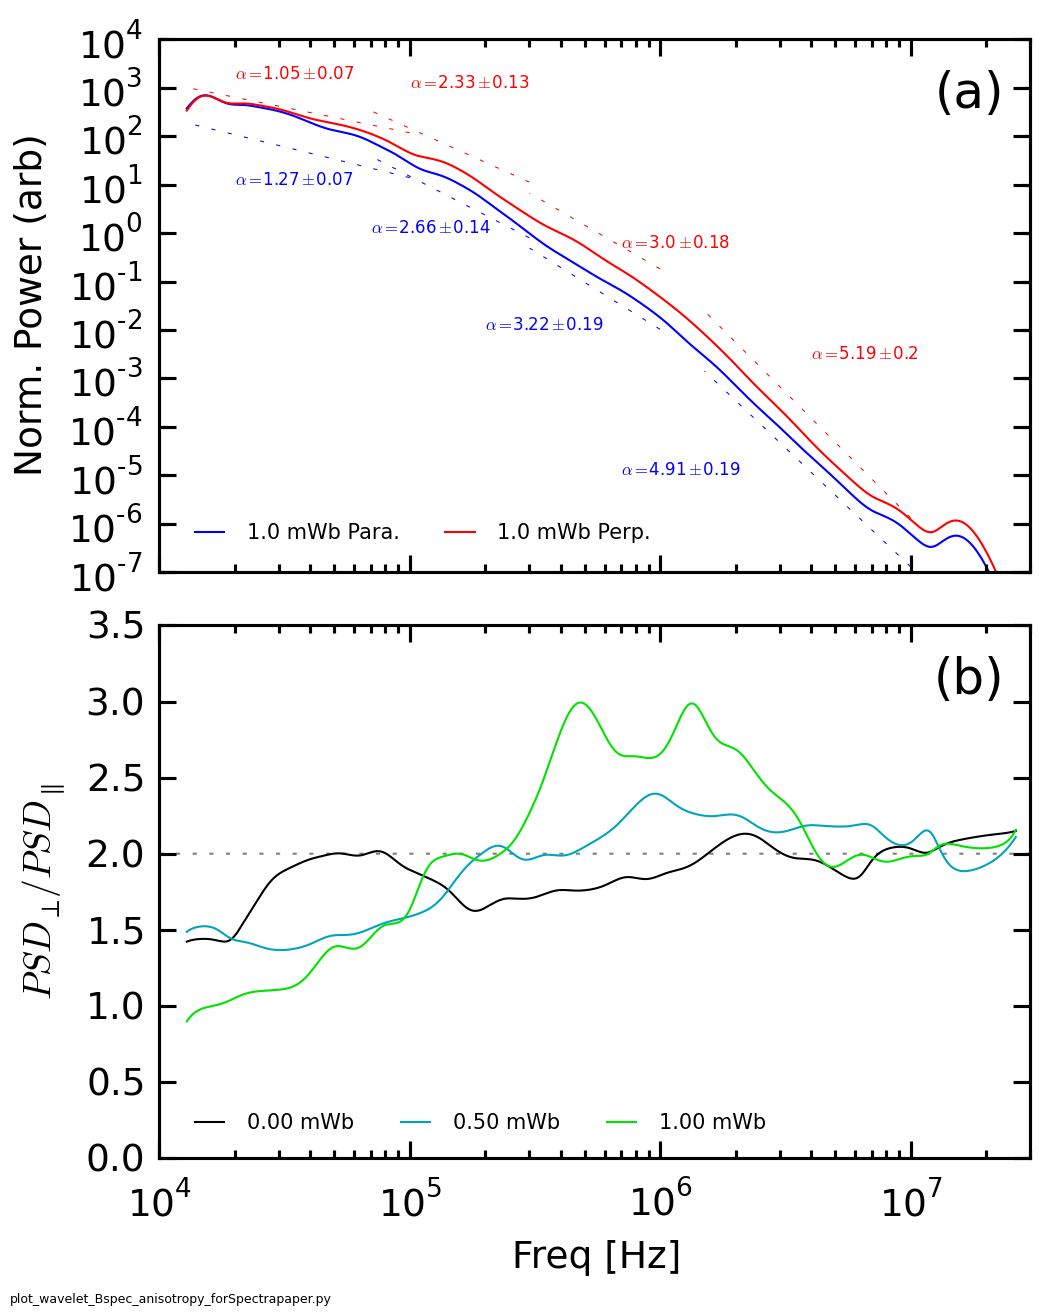
\includegraphics[width=8.5cm]{Bperppara_chan1t4_1mWbspectra_40t60us_wAsymRatio}}
\caption{\label{fig:spectra}}
\end{figure}

However, the separation between perpendicular and parallel spectra proceed in a manner similar to that found in space. Both perpendicular fluctuations (red) and parallel fluctuations (blue) begin at roughly the same magnitude in power. Beyond 20kHz, though, the parallel curve dips down slightly faster than the perpendicular and this trend continues up to about 500kHz. Then the separation begins to decrease and approaches a constant value from 5MHz to the Nyquist limit of 32MHz. This gradual change as a function of frequency is more clearly observed in figure ~\ref{fig:spectra}(b) plotted in log-linear format, which provides the ratio of the two curves in figure~\ref{fig:specta}(a). Since the fluctuations perpendicular to the B-field have two component directions while parallel fluctuations have only one, the point of isotropy, or equal fluctuations in all three components) occurs when the ratio of perpendicular to parallel equal to 2. Isotropy is indicated in figure~\ref{fig:spectra}(b) by the dashed gray line.

At the lowest frequencies, the balance of power actually tips toward parallel over perpendicular. As the frequency decreases, an thus, presumably, the scale size decreases, the ratio approaches isotropy, then changes over to a dominantly perpendicular power level. The ratio continues to steadily increase reaching a peak of about 3 at about 500kHz. There is a brief dip before the ratio rises again at about 1.5MHz; at this point, the ratio begins to drop steadily, and approaches an isotropic level at about 5MHz. 

The scale dependency of the 1.0mWb data can be compared to other helicity levels. The black curve shows the anisotropy ratio for the zero helicity state, when the field strength is about an order of magnitude less, and there is much less structure to the field. As might be expected for such a state, there appear to be very little anisotropy at any scale with values staying close to R=2. The blue curve, showing the anisotropy ratio for a 0.5mWb stuffing case, clearly shows intermediate ratios between the 1.0 and 0.0mWb plasmas. This observation is somewhat curious as there is very little difference in magnetic field magnitude between 1.0mWb and 0.5mWb; the only difference between to the two states is the amount of average flow (which would not be expected to affect anisotropy) and the amount of helicity in the plasma.

\begin{figure}[!htbp]
\centerline{
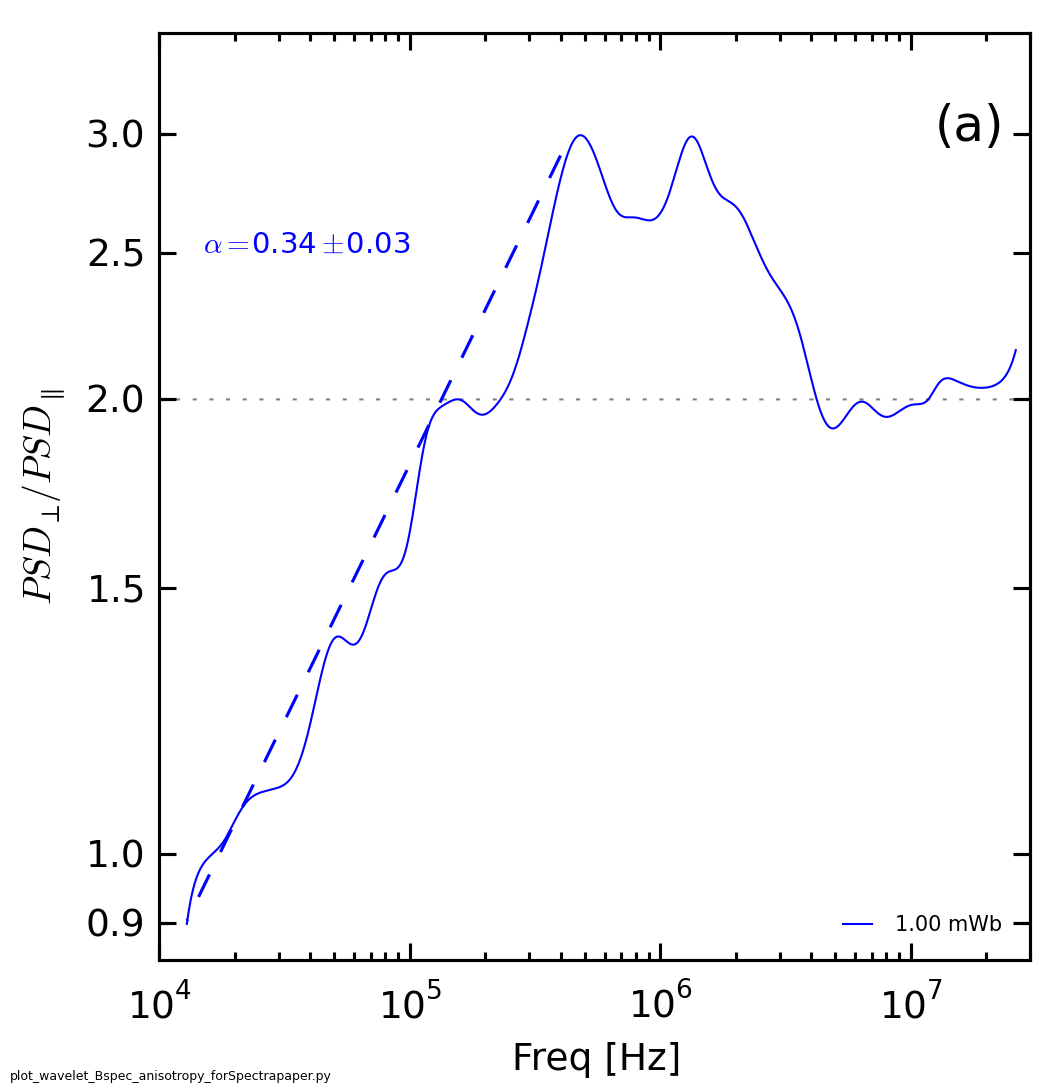
\includegraphics[width=8.5cm]{Bperppara_chan1t4_1mWbspectra_40t60us_AsymRatio_wFit}}
\caption{\label{fig:fitratio}}
\end{figure}

\begin{figure}[!htbp]
\centerline{
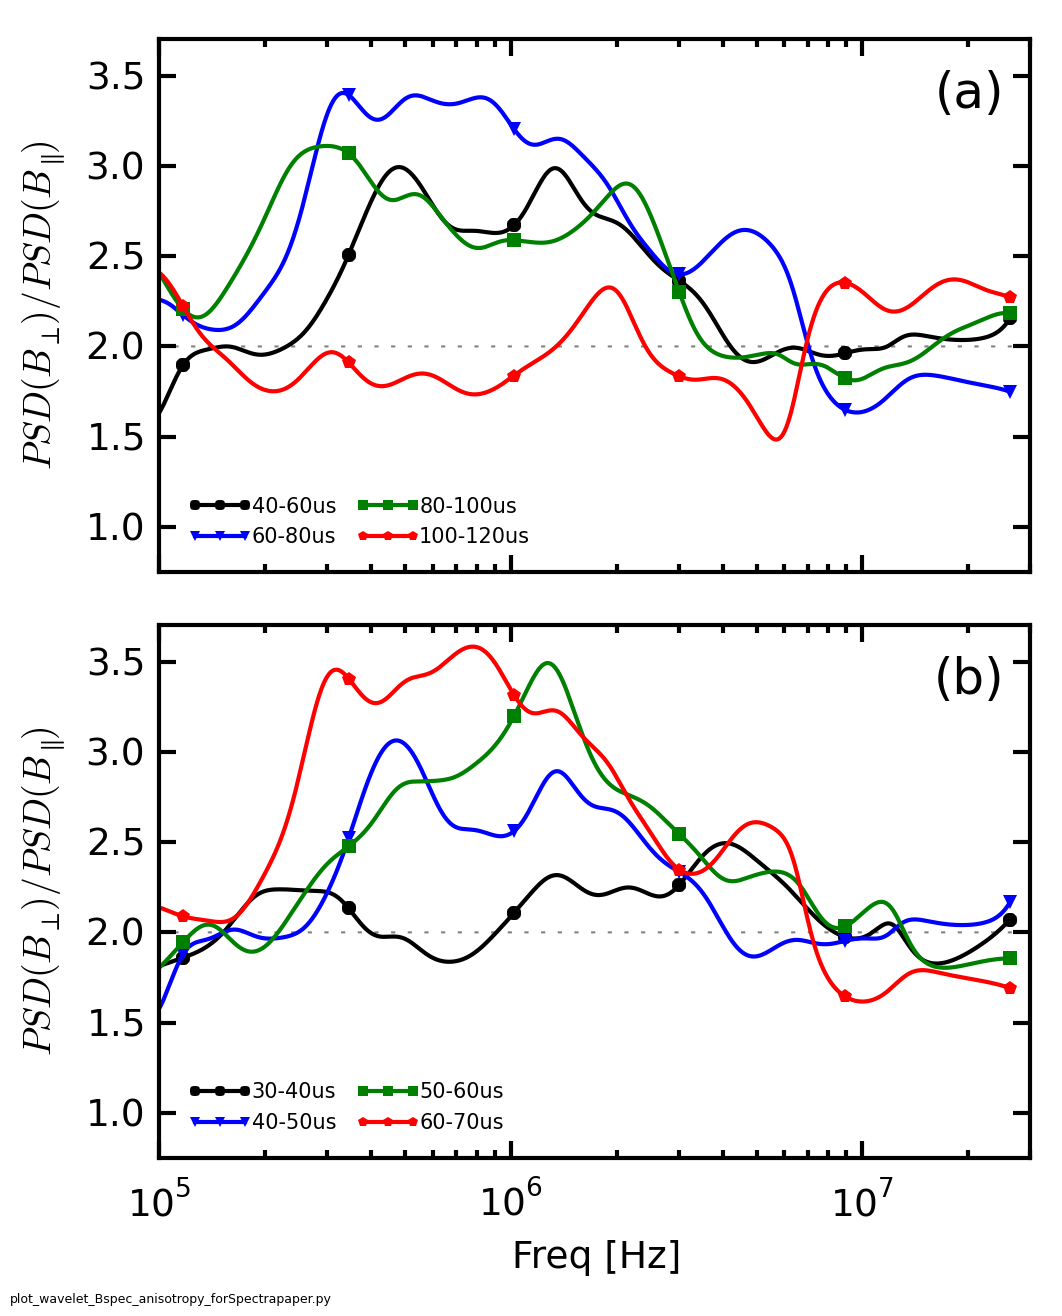
\includegraphics[width=8.5cm]{Bperppara_chan1t4_1mWbspectra_timescan}}
\caption{\label{fig:timeratio}}
\end{figure}

Fits to both the spectra and the ratio are shown in figure~\ref{fig:spectra}. In figure~\ref{fig:spectra}(a), fits are made to four sections of each curve. The spectral indices, error and range of fit for both parallel and perpendicular spectra are shown in the table below. Overall, the spectral indicies are anisotropy; for each section fit, the parallel slope is consistently steeper than the perpendicular slope. This difference is also reflected in the fit shown in figure~\ref{fig:fitratio}. An index of $\alpha = 0.35$ indicates that the ratio scales like $f^{1/3}$ for the region between 10kHz and 500kHz.

An evolution of the anisotropy over time is also observed. Figure~\ref{fig:timeratio}(a) and (b) shows the change of the anisotropy ratio as a function of time ranges of 10$\mu s$ intervals(a) and 20$\mu s$ intervals(b). The black curve in figure~\ref{fig:timeratio} shows a period of time, 30-40$\mu s$, just as the plasma is reaching the midplane probe. The curve remains near isotropic levels for most of the frequencies. As time increases in 10$\mu s$ intervals, the perpendicular power clearly increases in the 100kHz to 1MHz range, while decreases in the 10-100kHz range. The actually peaks highest in the time frame just beyond the main analysis period shown in figure~\ref{fig:spectra}(b). These trends demonstrate that the anisotropy increases as more time is allowed for the turbulence to evolve. Figure~\ref{fig:timeratio}(b), shows that after energy is no longer being injected to maintain the turbulence, the anisotropy decreases. After 100$\mu s$, the magnetic field fluctuations have return to isotropy.

\section{Flow and Density Spectra}

For a turbulence cascade to develop, a system needs both energy injection and energy dissipation. The separation of spatial scale between injection and dissipation determines the size of the inertial range. While the actual injection mechanisms of the solar wind are not completely understood, there is evidence from the comparison of large scale magnetic field and velocity fluctuation data that velocity fluctuation energy is being tapped by magnetic fluctuations to sustain an injection-range like cascade for magnetic spectra~\cite{roberts10}. In the SSX plasma, however, the injection scale energy is primarily magnetic---the formation of the unstable spheromaks. This is borne out by similar comparisons of magnetic spectra and velocity spectra. Figure~\ref{fig:BvsFlow} shows magnetic spectra (a) and Mach number fluctuation spectra (b) for two plasma states: a high and low magnetization state.

\begin{figure}[!htbp]
\centerline{
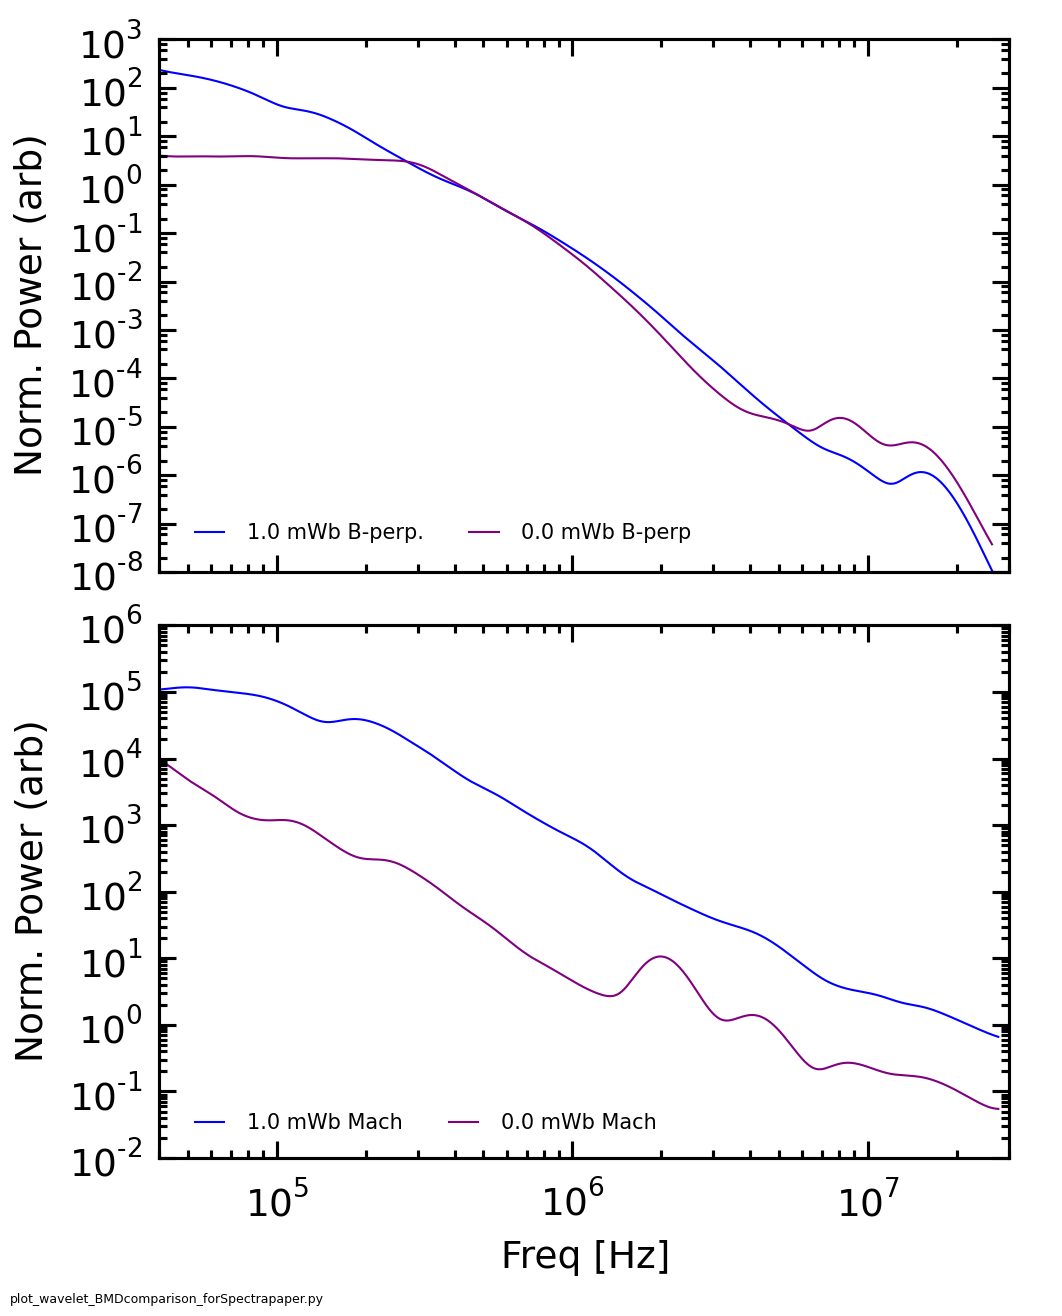
\includegraphics[width=8.5cm]{BvsFlowspec_2fluxes_separateplots_40t60us}}
\caption{\label{fig:BvsFlow}}
\end{figure}

Comparison of the blue and purple curves in Figure~\ref{fig:BvsFlow}(a) show the affect on large scale fluctuations from the presense of a strong initial magnetic field. Comparing these states with the respective velocity fluctuations shows how the additional magnetic energy injection at larger scales affects the velocity. For the low field state, the velocity cascade is immediately steep as well as lower in energy overall. In the high field state, however, the velocity fluctuation scaling is shallower, but then has a breakpoint around the frequency where B-field fluctuation energy is about the same between high and low field states. This suggests that the state with more injected magnetic energy delivers some of its energy to the velocity fluctuations.

\begin{figure}[!htbp]
\centerline{
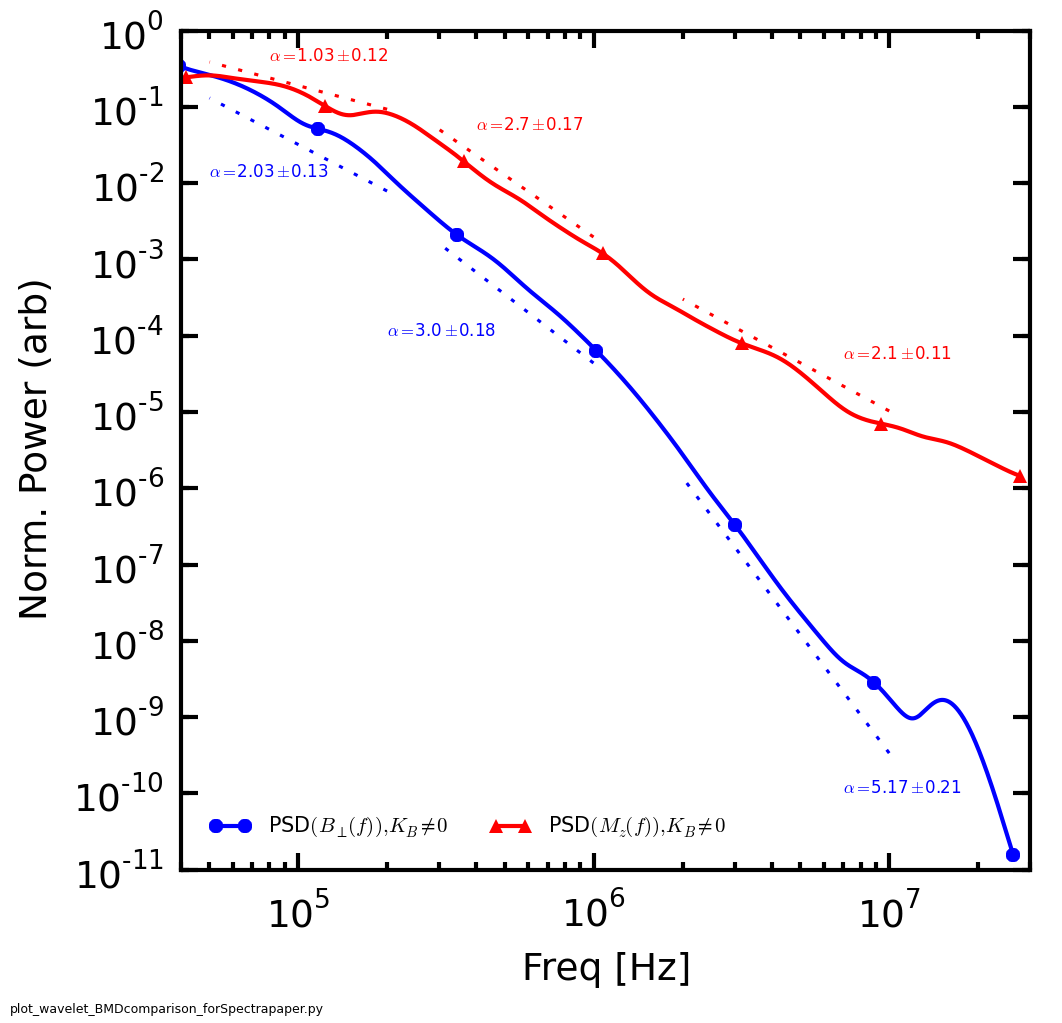
\includegraphics[width=8.5cm]{BvsFlowspec_wFits_40t60us}}
\caption{\label{fig:BvsFlow_wFits}}
\end{figure}

This can be seen quantitatively in Figure~\ref{fig:BvsFlow_wFits} which puts the high field magnetic and velocity fluctuation spectra on the same relative scale. The velocity spectra scales like $f^{-1}$ about to about 200kHz, a scaling which is typical for injection range turbulence. Meanwhile, the magnetic spectra is steeper, which implies that some of the magnetic energy may be going to drive flows, though the exact mechanism of this energy transfer is not known and its study is reserved for later work.

Beyond 200kHz, the velocity fluctuations scaling steepens suggesting an inertial range scale. The B-field steepens further as well. Beyond, 2MHz, the B-field scaling drops off significantly while the velocity spectra scaling actually slightly increases. This is possibly due to a dissipation mechanism that may be further tapping magnetic energy, and given the increase in velocity spectra scaling, even further adding to velocity fluctuation energy. It may, however, also be due to the frequency of response of the Mach probe itself. Alternative velocity fluctuation measurements are being considered (i.e. electric field fluctuations) for future runs for comparison.

\section{Wavenumber Spectra}

A unique turbulence measurement that can be made in the SSX plasma is a direct wavenumber spectrum using a multi-tipped magnetic probe that is inserted radially into the wind-tunnel. The probe can measure $\vec{B}(t)$ at 16 locations along a 6.8cm length of the radius at a spacing of 0.4572cm. In Fourier space, this allows measurements of scales from about 7cm to 1cm. Given that the injection scale of the magnetic energy is on the order of the initial size of the spheromaks---15.5cm---and a dissipation scale can be estimated to be just under 1cm---ion inertial length for a 1.5$\times 10^{15}$cm$^{-3}$ plasma is on the order of 0.6cm---the spatial range sampled by the probe can be assumed to be in the inertial range.

Since the probe can take simultaneous measurements of $\vec{B}$ across the plasma, snapshots of the spatial structure of the plasma can be made at each time step. In turn, these spatial distributions can be Fourier transformed to produced power-spectra of the scales. Thus, this measurement can capture the direct wavenumber spectra of the plasma turbulence without reliance on any Doppler shifting as is needed to invoke the Taylor Hypothesis. Moreover, since $\vec{B}$ is constructed from three orthogonal measurements, the power-spectra of vectors perpendicular and parallel to the axial flow of the plasma can be separately analyzed. 

The downside, of course, to a measurement of the wavenumber spectra in this way is the lack of resolution compared to a Doppler-shifted frequency spectrum. With only 16 spatial points, the Fourier spectrum can have only 8 points, and only seven can be displayed in log-log format. However, despite this lack of resolution, it is a more physical direct measurement and can the measurement can still be used to cross-reference other observations of spectra.

\begin{figure}[!htbp]
\centerline{
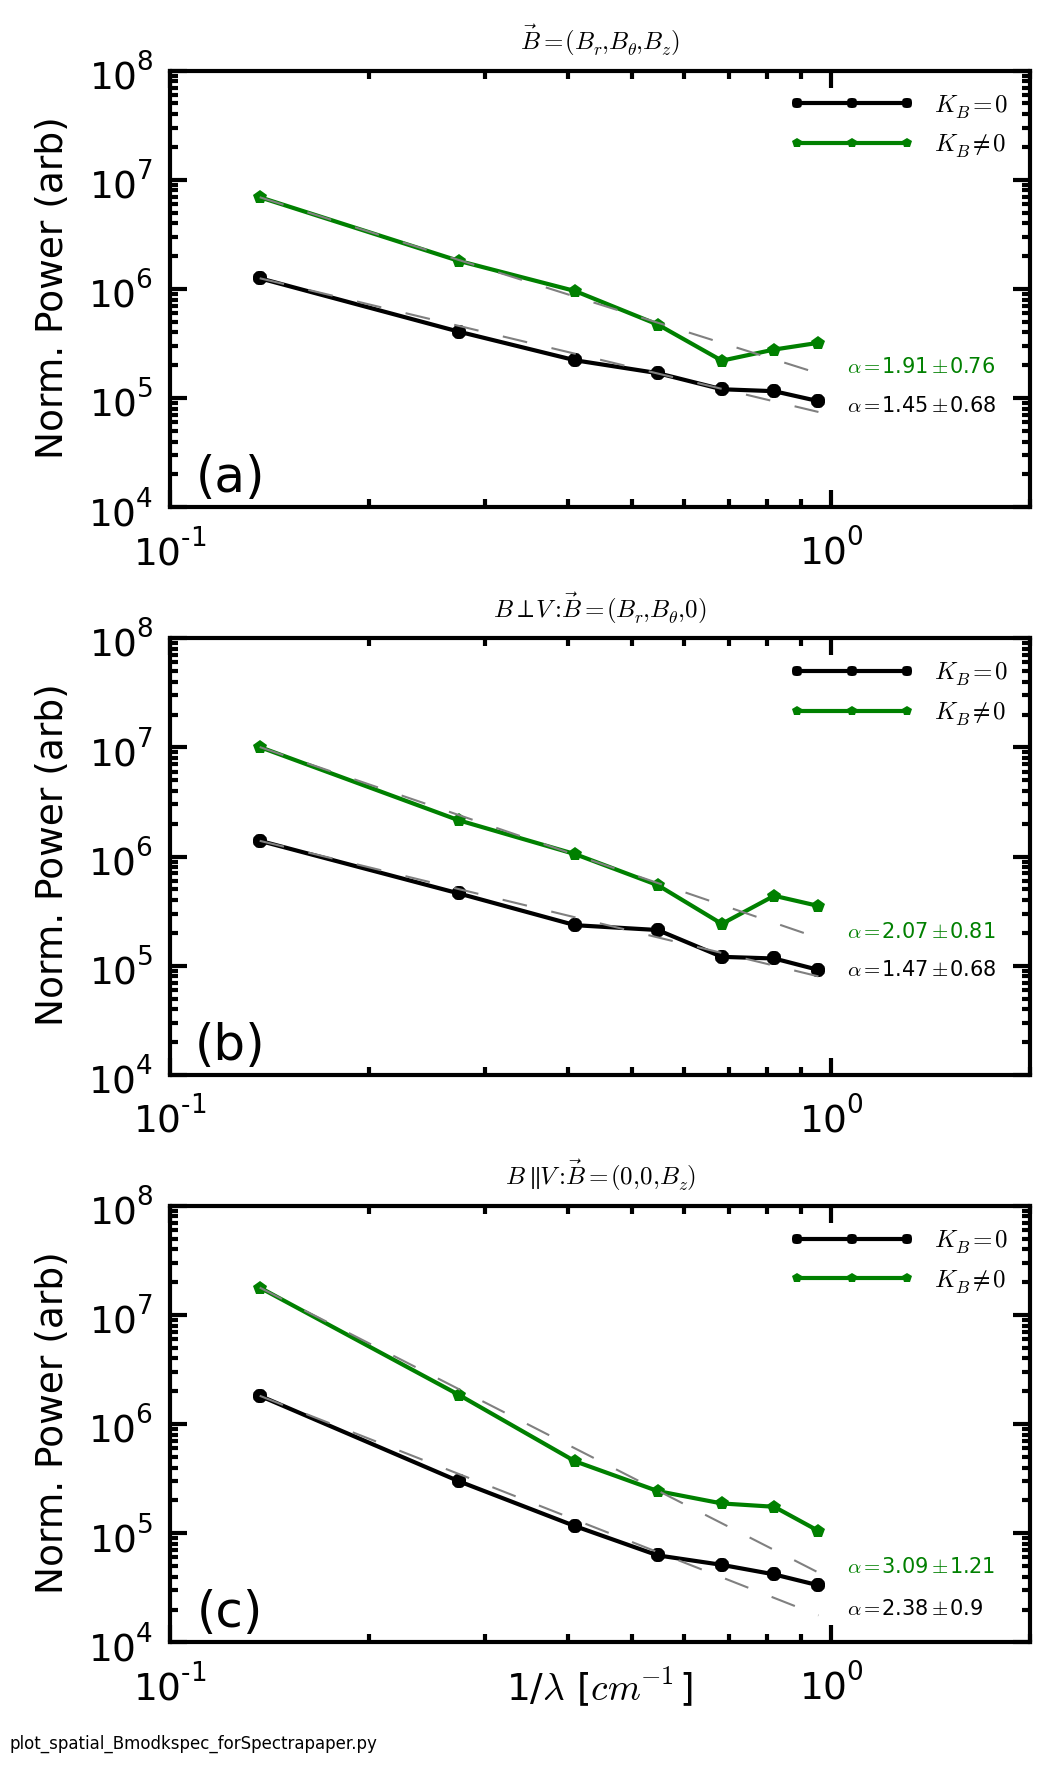
\includegraphics[width=8.5cm]{Bmod_FFTwavenumberspectra_wFits_40t60us}}
\caption{\label{fig:wavenumber_spectra}}
\end{figure}

Figure~\ref{fig:wavenumber_spectra} shows the wavenumber power spectrum for three different helicity states and for full-vector(a), perpendicular vector(b) and parallel vector(c), averaged for each timestep in between 40 and 60$\mu s$ and over 40 shots. Comparison of the three curves in Figure~\ref{fig:wavenumber_spectra}(a) seem to show a slight variation in slope as the helicity state is increased, though with the large given errors in the fit (due to low resolution), the slopes of all three curves are essentially the same. A similar trend is observed amongst the three curves in (b) and (c) as well. A larger difference arises when comparing the curves of different vectors. Namely, the separately computed perpendicular and parallel spectra in (b) and (c) tend to be slightly steeper than the full vector spectra in (a). Moreover, the parallel curves appear to be steeper than the perpendicular curves. Again, the error in the fits are large for the low resolution data, but the trends are very suggestive.

\begin{figure}[!htbp]
\centerline{
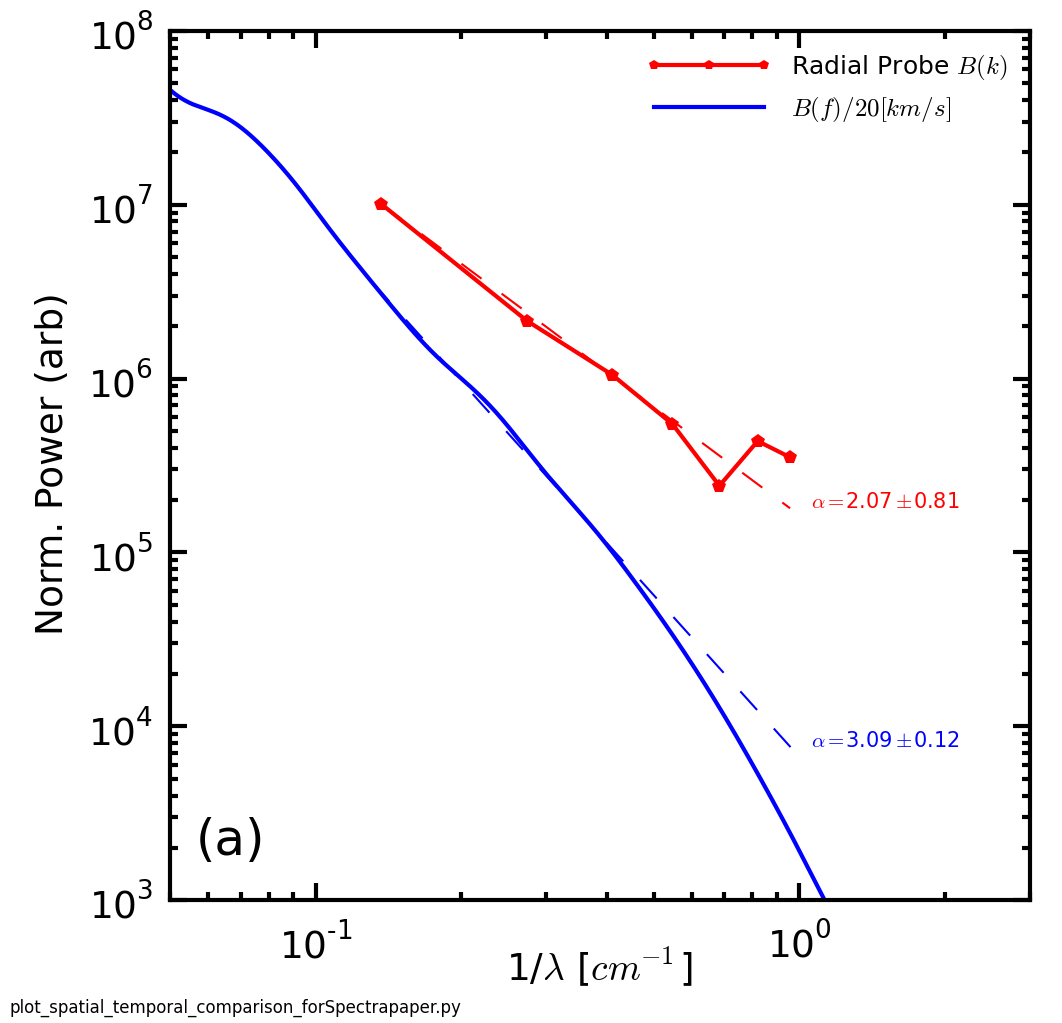
\includegraphics[width=8.5cm]{B_spatial_temporal_comp_wFits_40t60us}}
\caption{\label{fig:wavenumber_comp}}
\end{figure}

The wavenumber spectra and frequency spectra can be directly compared by invoking the Taylor hypothesis for the frequency spectra and Doppler-shifting the frequency spectra by the bulk plasma velocity,
\begin{equation}
B(f) \longrightarrow B(f-kV_{p}) \longrightarrow \frac{1}{V_{p}}B(k)
\label{eq:Taylor_Hyp}
\end{equation}

For this plasma, the velocity can be estimated (using both time-of-flight and Mach probe measurements) to be about 20km/s. If the frequency portion is ignored in Equation~\ref{eq:Taylor_Hyp}, the frequency spectra can be plotted on the same scale as the wavenumber spectra. Figure~\ref{fig:wavenumber_comp} shows this comparison for the 1mWb stuffing flux plasma. The curves are placed arbitrarily on the y-axis. Maximum likelihood estimation power-law fits are made to the same range in both curves. The slopes of the curves are comparable suggesting that invoking the Taylor hypothesis for the frequency spectra is not entirely unwarrented. Instead, the steeper slope of the frequency spectra could be reflective of the effect of a combined temporal {\it and} spatial scaling, which the direct wavenumber spectrum does not include. However, breakdown of Taylor Hypothesis has been shown to make the spectra more shallow than steeper(Klein Taylor Hypotheis draft). The differences might also be reflective of a wavenumber anisotropy as the direct wavenumber spectra probes $k_{r}$ and the Doppler-shifted frequency spectra probes $k_{z}$.

\section{Comparison with Simulation}

Simulations of the plasma produced in the SSX wind-tunnel have been generated with the HiFi spectral-element multi-fluid modeling framework using a set of normalized compressible Hall-MHD equations. Favorable comparisons of turbulent spectra and intermittency have been reported between these simulations and the experimental plasma~\cite{schaffner14a}. Further analysis is presented here which show similar observations of anisotropy, wavenumber spectra, and velocity-B-field spectra comparisons as is seen in the experiment.

Timeseries of quantities in 3mm spheres approximately 1cm off the central axis and at the midplane are extracted from the simulation for density, three axes of magnetic field, three axes of velocity. To provide some ensemble averaging, points at eight different azimuthal angles are used.

\begin{figure}[!htbp]
\centerline{
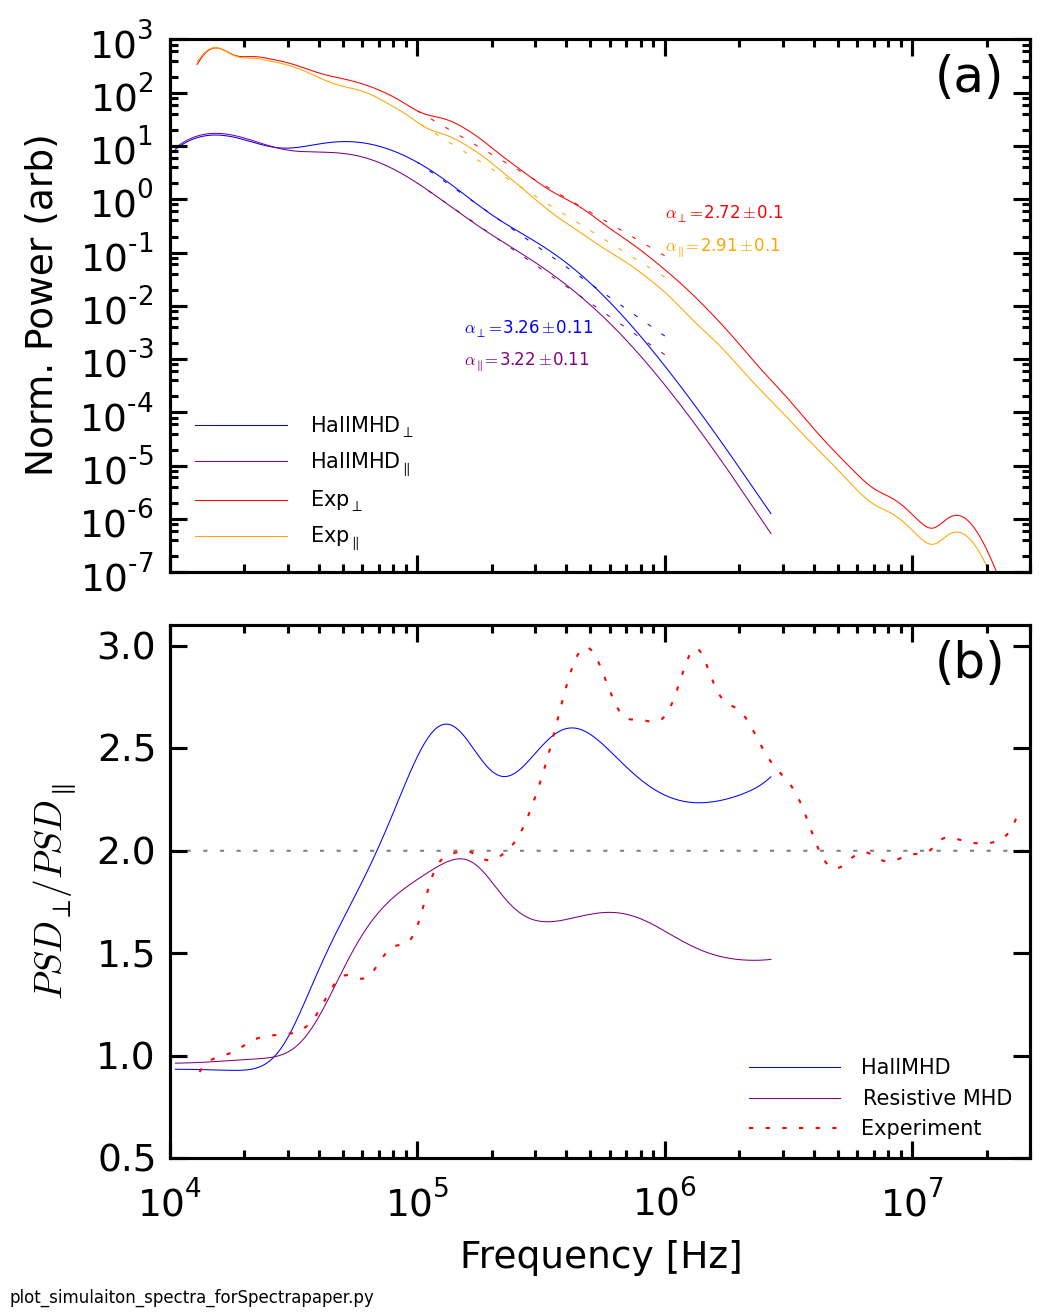
\includegraphics[width=8.5cm]{Anisotropy_simulation_comparison}}
\caption{\label{fig:aniso_comp}}
\end{figure}

The simulation timeseries data is analyzed in a similar was the the experimental data with the exception that the mother wavelet used for the wavelet transform of the simulation data is a fourth-order Paul rather than a sixth-order Morlet, in order to better capture time resolution for the lesser sampled simulation. A variance anisotropy analysis is conducted in the same manner as well using a local magnetic field and the projection method. Figure~\ref{fig:aniso_comp}(a) shows simulation decomposition into perpendicular and parallel spectra compared to experimental spectra using the 1.0mWb stuffing data. The simulation and experimental spectra are staggered placed on the y-axis to emphasize features of the shape. Clearly, the simulation data exhibits growing variance anisotropy with increasing frequency. The slopes of the simulation spectra match qualitatively well in the region of 100kHz to 1MHz, though the fit spectra indices indicate a slightly steeper slope than the experiment. The high frequency end of the simulation spectra drops in power faster than the experiment, likely due to the limits in time resolution.

The trend in anisotropy ratio is also similar in the simulation and the experiment, as seen in Figure~\ref{fig:aniso_comp}(b), though the simulation does not reach as large a peak ratio, nor does it scale at quite the same rate. Nevertheless, the clear observation of increase an increase in ratio suggests that the compressible Hall-MHD physics captures the generation of the anisotropy. Figure~\ref{fig:aniso_comp}(b) also shows the anisotropy ratio for a simulation run with the Hall term in the compressible MHD equations set to zero. Unlike the Hall MHD and the experiment, the ratio does not switch over to perpendicular dominance, and instead stays near or below the isotropy line. The implications of this have not been analyzed in depth.

\begin{figure}[!htbp]
\centerline{
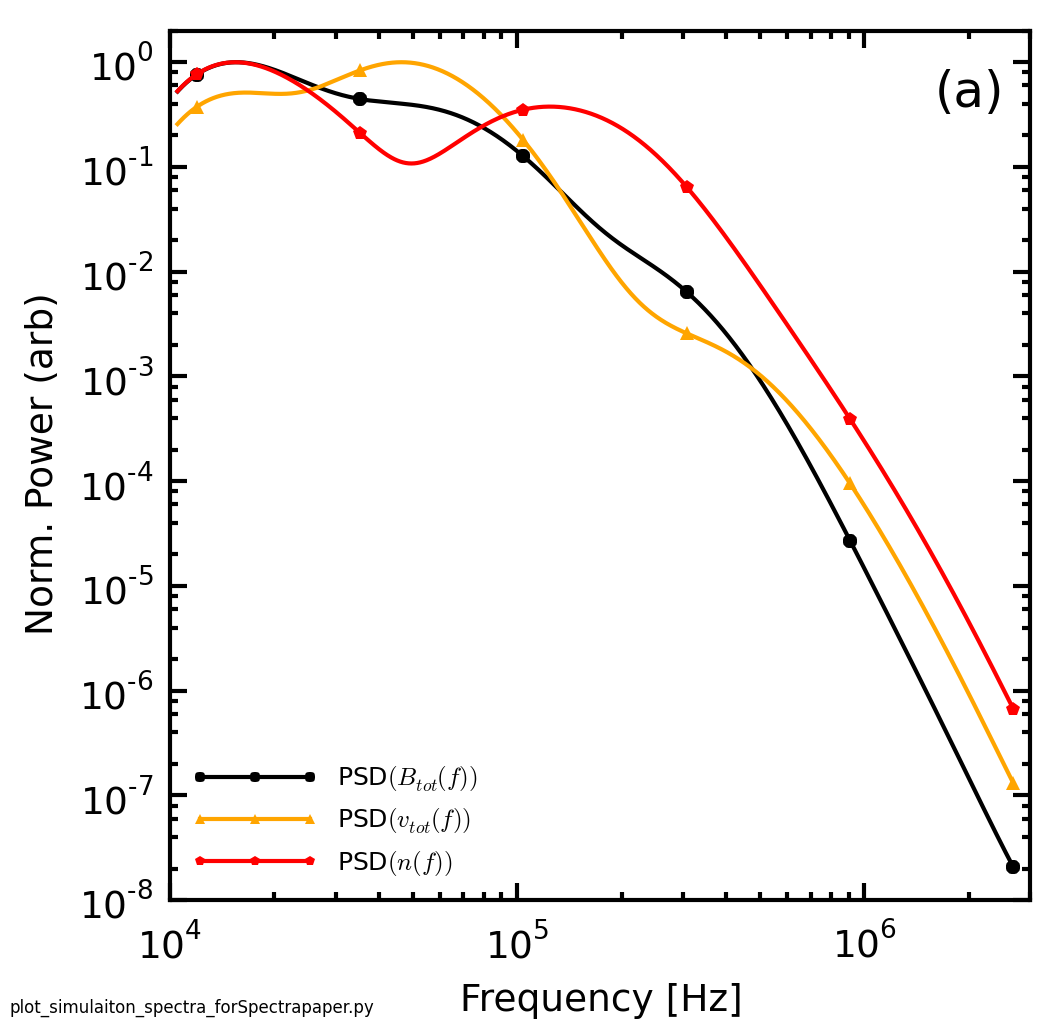
\includegraphics[width=8.5cm]{BfieldFlow_simulation_comparison}}
\caption{\label{fig:bflow_comp}}
\end{figure}

A comparison between velocity and magnetic field fluctuations in the simulation can also be made. Figure~\ref{fig:bflow_comp} shows wavelet transformed frequency power spectra for the total magnetic field (sum of $B_{r}$, $B_{\theta}$, and $B_{z}$), total velocity, and density, all normalized to their respective peaks. Qualitatively, the comparison between velocity and magnetic field spectra supports the results of the experimental data for stuffed plasmas: the peak in the velocity spectra occurs at a larger frequency than the magnetic spectra. This suggests that energy for the velocity fluctuations are being injected at a smaller scale than the magnetic field fluctuations. Though not conducted here, further analysis of the simulation could potentially show direct energy transfer between the magnetic and velocity fluctuations.

\begin{figure}[!htbp]
\centerline{
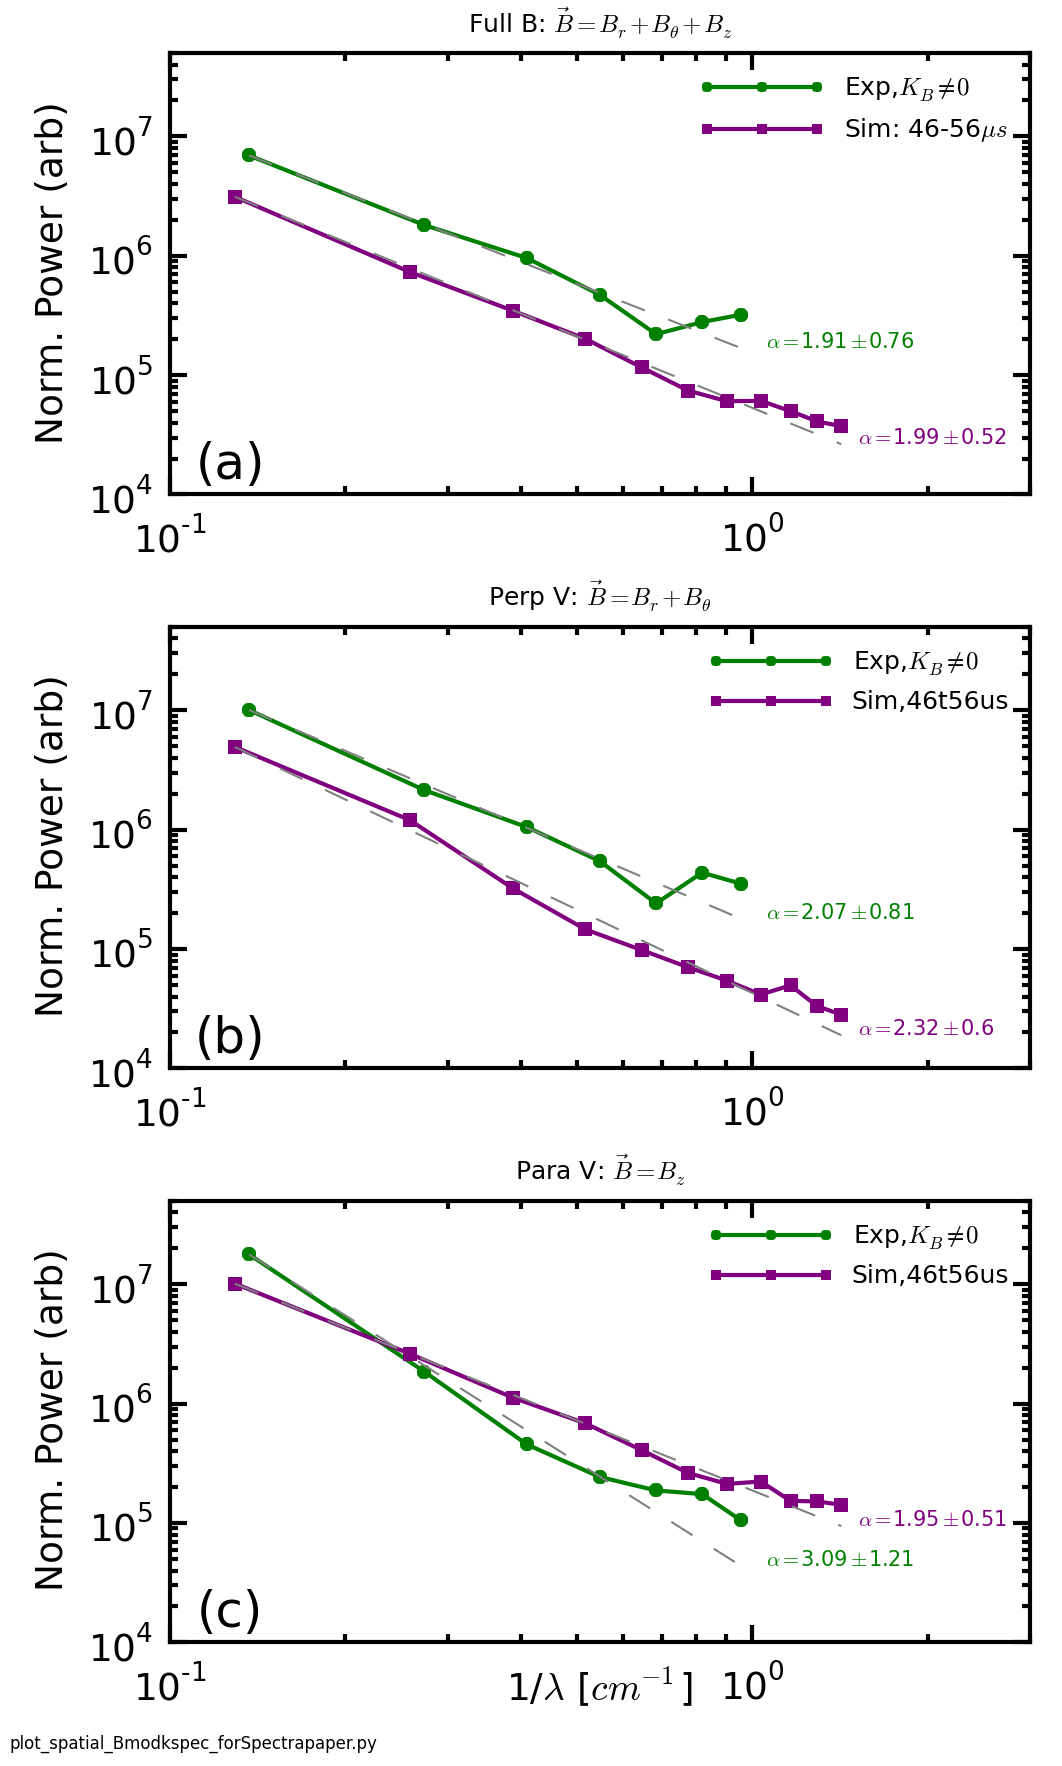
\includegraphics[width=8.5cm]{Bmod_FFTwavenumberspectra_wFits_40t60us_simulationcomparison}}
\caption{\label{fig:sim_wavenumber_comp}}
\end{figure}

\begin{figure}[!htbp]
\centerline{
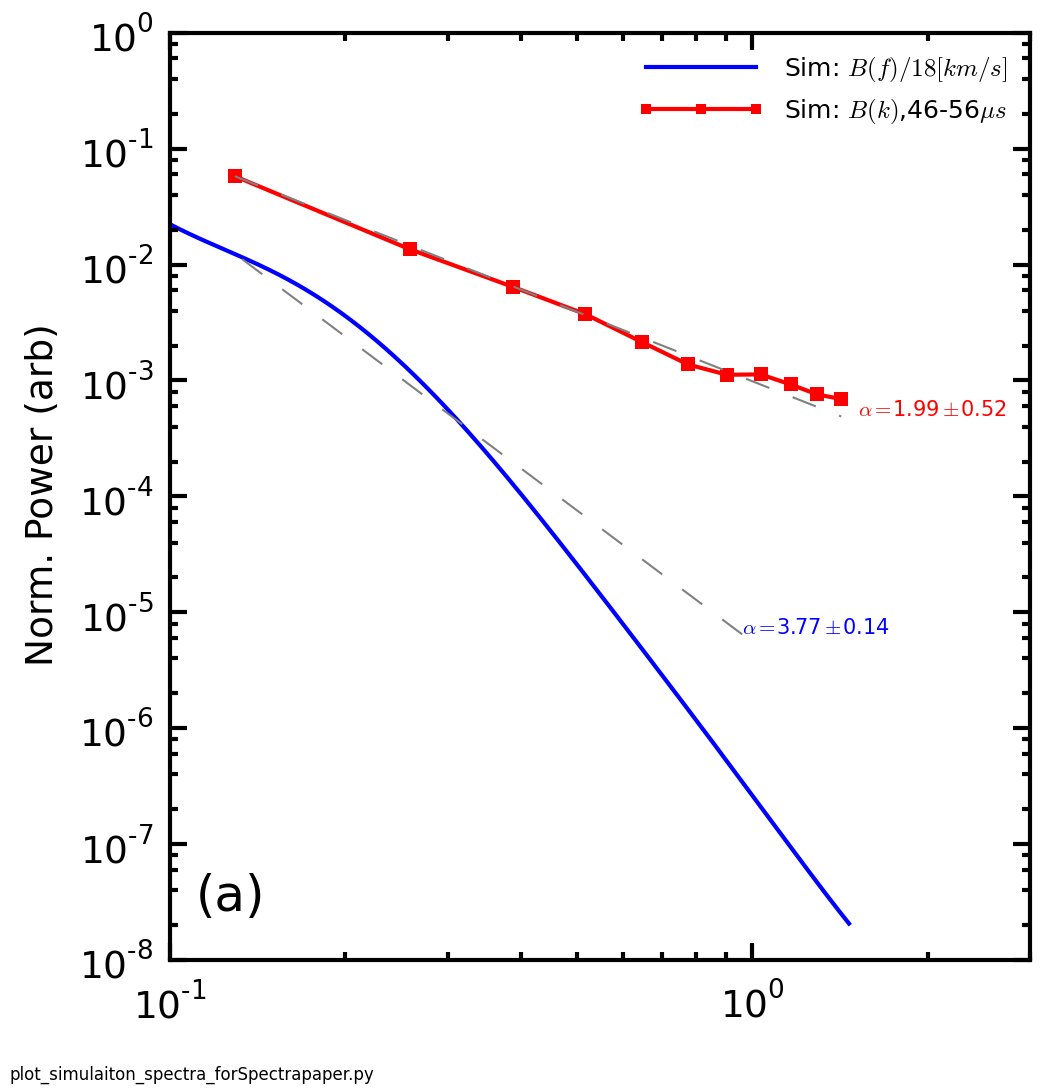
\includegraphics[width=8.5cm]{Simulation_spatial_temporal_spectra_comparision}}
\caption{\label{fig:sim_spatial_comp}}
\end{figure}

The wavenumber spectra from a radial cut of the simulation data is also generated using 24 points. Figure~\ref{fig:sim_wavenumber_comp} shows a direct comparison between simulation and experimental wavenumber spectra. The slightly smaller separation between distances allows the simulation to reach a smaller scale than the experiment, to about 0.7cm. In general, the comparison between simulation and experiment is good suggesting that the simulation is capturing well the spatial structure of the turbulence. Even though the simulation can observe slightly smaller scales, it does not appear to probe small enough to exhibit any dissipation effects at to ion inertial length scales which for the simulation is at about 0.7cm.

Like in the experiment, the spatial and temporal spectra of the simulation is compared and shown in Figure~\ref{fig:sim_spatial_comp}. The simulation has a bulk axial flow of 18km/s, close to the 20km/s observed in the experiment. A similar trend is seen with the spatial spectra having a shallower slope than the Doppler-shifted frequency spectra. The main difference again appears to be that the frequency spectra hits the limits of the temporal resolution at larger frequencies than the experiment.

These further comparisons of turbulent statistics and characteristics between the experimental plasma and a compressible Hall-MHD simulation help validate the model as useful for understanding the physical processes. Subsequent simulation analysis will likely entail more detailed computation of how energy might be being distributed and moved through the plasma including relationships between magnetic field and velocity as well as between magnetic fluctuations perpendicular and parallel to a local B-field.

\section{Discussion and Evidence for Ion Scale Effects}

\begin{figure}[!htbp]
\centerline{
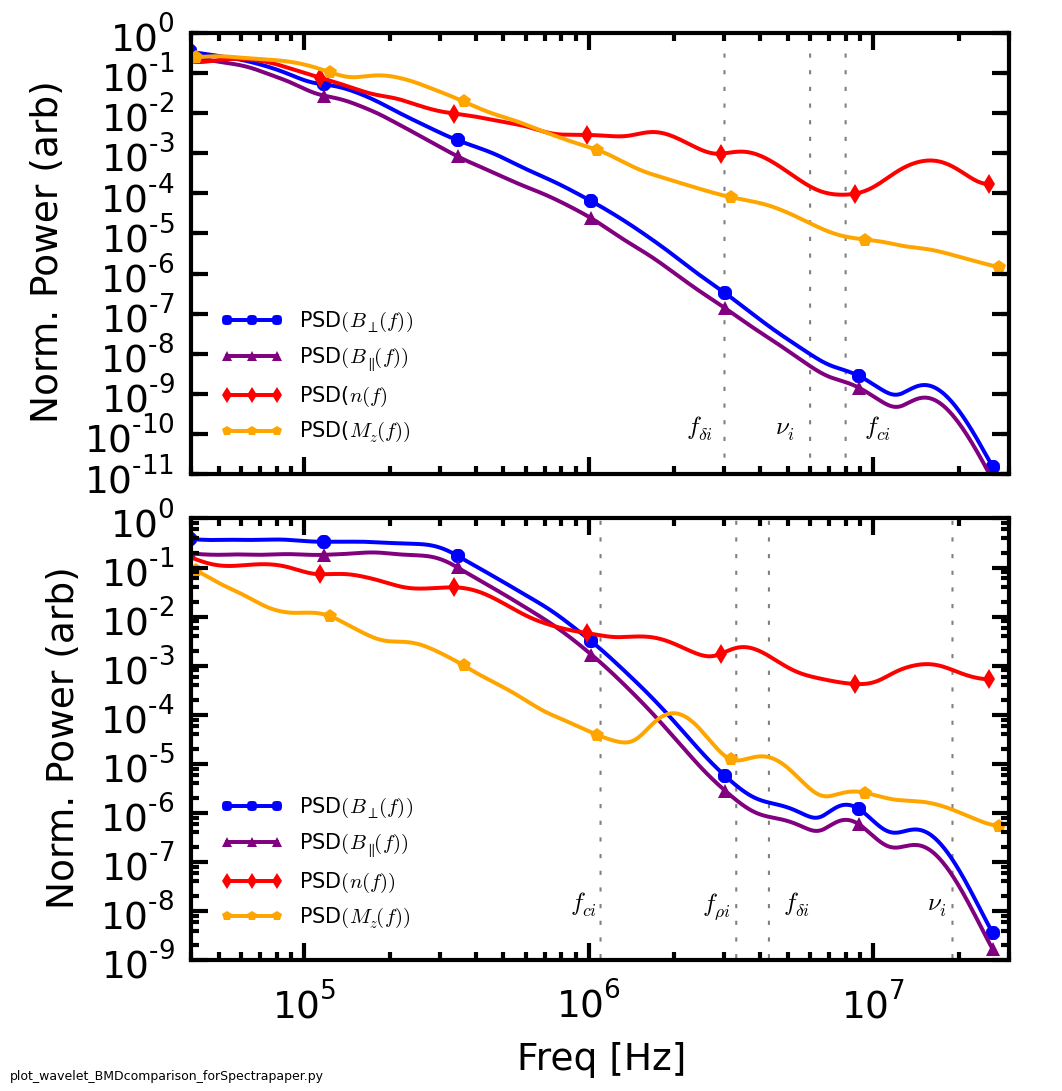
\includegraphics[width=8.5cm]{BvsDensvsFlowspec_1mWb_and_0mWbcomp_40t60us}}
\caption{\label{fig:BMD_comp}}
\end{figure}

%1mWB run
%dens 1.39e15 cm^-3
%bfield 5283 G
%Ti = 23 eV
%bulk flow = 20km/s

%results
%Va = 309km/s
%Beta = 0.07
%Cs = 31km/s
%f_i = 8MHz
%nu_i = 6MHz
%rho_i = 0.09cm
%c/w_pi = 0.61cm
%ion_mfp = 0.16cm
%doppler shifted c/wpi = 3MHz
%doppler shifted rho_i = 20MHz

%0mWb run
%dens 2.84e15 cm^-3
%bfield 747 G
%Ti = 17 eV
%bulk flow = 20km/s

%results
%Va = 30km/s
%Beta = 5.5
%Cs = 31km/s
%f_i = 1.1MHz
%nu_i = 19MHz
%rho_i = 0.56cm
%c/w_pi = 0.43cm
%ion_mfp = 0.05cm
%doppler shifted c/wpi = 4.3MHz
%doppler shifted rho_i = 3.3MHz

\begin{table}
\caption{\label{tab:params}MHD wind tunnel plasma parameters during the equilibrium epoch for the present configuration of SSX.}
\begin{tabular}{|l|l|l|}
\hline
Parameter&1.0mWb&0.0mWb\\
\hline
$Measured$&&\\
\hline
$\langle |B|\rangle [kG]$&5.283&0.747\\
$\langle n\rangle \times 10^{15} [cm^{-3}]$&1.39&2.84\\
$\langle T_{i}\rangle [eV]$&23&17\\
Bulk Flow $[km/s]$&20&20\\
\hline
$Computed$&&\\
\hline
$\beta$&0.07&5.5\\
$V_{a} [km/s]$&309&30\\
$C_{s} [km/s]$&31&31\\
$\rho_{i} [cm]$&0.09&0.56\\
$\delta_{i} [cm]$&0.61&0.43\\
$\lambda_mfp^{i} [cm]$&0.16&0.05\\
$f_{ci} [MHz]$&8&1.1\\
$\nu_{i} [MHz]$&6&19\\
$f_{\delta i} [MHz]$&3&4.3\\
$f_{\rho i} [MHz]$&20&3.3\\
\hline
\end{tabular}
\end{table}

A major remaining question for this analysis is whether the plasma diagnostics are able to observe effects of a dissipation scale in this turbulence. Perhaps, a more general question can be posed in how well does this plasma exhibit a traditional fluid-turbulence-like picture which posits an injection scale, inertial scale and dissipation scale.

\section{Conclusions}

\appendix

\section{Computation of Variance Anisotropy}

The computation of the variance anisotropy involves two main steps: a determination of fluctuation power and an estimate of the distribution of the fluctuation power relative to a vector direction. The first step is accomplished using a Wavelet transform procedure as is discussed in the text. The division of fluctuation power is accomplished using what will be described here as a projection method. A second estimate of fluctuation power distribution is constructed using a threshold method and is also described in detail in this appendix. The threshold method is a more straightforward process for determining the level of variance anisotropy, but suffers from diminishing resolution. Its presentation here is mainly as a validation of the eventual use of the projection method for the analysis in the paper. 

\subsection{Threshold Method}

Both the threshold method and the projection method for determining variance anisotropy rely on the ability of the wavelet transform to yield a power spectrum distribution (PSD) as a function of both time and frequency (i.e. B(f,t)). A local (in time) vector $\vec{B}$ is determined for each time, t,
\begin{equation}
\vec{B}(t) = B_{r}(t)\hat{r} + B_{\theta}(t)\hat{\theta} + B_{z}(t)\hat{z}
\label{eq:Bvector}
\end{equation}
where each component $n=r,\theta,z$ is determined from $\dot{B}_{n}$ by integrating over time as
\begin{equation}
B_{n}(t) = \int_{0}^{t} \frac{d}{d\tau}B_{n}(\tau)d\tau.
\label{eq:Bintegrated}
\end{equation}

Since the magnetic probe measures orthogonal magnetic field directions by construction, this fact can be used to directly seek a difference in fluctuation spectra depending on orientation perpendicular or parallel to the overall field. Thus, a threshold magnitude for each component can be defined as a fraction of the total magnitude as in,
\begin{equation}
B_{n}^{threshold} \geq \frac{|B_{n}|^{2}}{|\vec{B}|^{2}}
\label{eq:Bthreshold}
\end{equation}
which reflects the relative amount that the total vector points in one of the three orthogonal directions. Then for every time, t, in a given time range and for each shot, the quantity $B_{n}(f,t)$ is summed for each t where
\begin{equation}
\frac{|B_{n}|^{2}}{|\vec{B}|^{2}} \geq B_{n}^{threshold}
\label{eq:Bcondition}
\end{equation}
for all frequencies, $f$. The value chosen for $B_{n}^{threshold}$ determines how strictly total vector aligns with the component, $n$. By definition, then, the summed power for $B_{n}$ is considered the parallel component and the sum of the remaining two directions is the perpendicular component. If there is any anisotropy in the signal, a difference in energy content of the spectra should become apparent as the threshold value is increased.

\begin{figure}[!htbp]
\centerline{
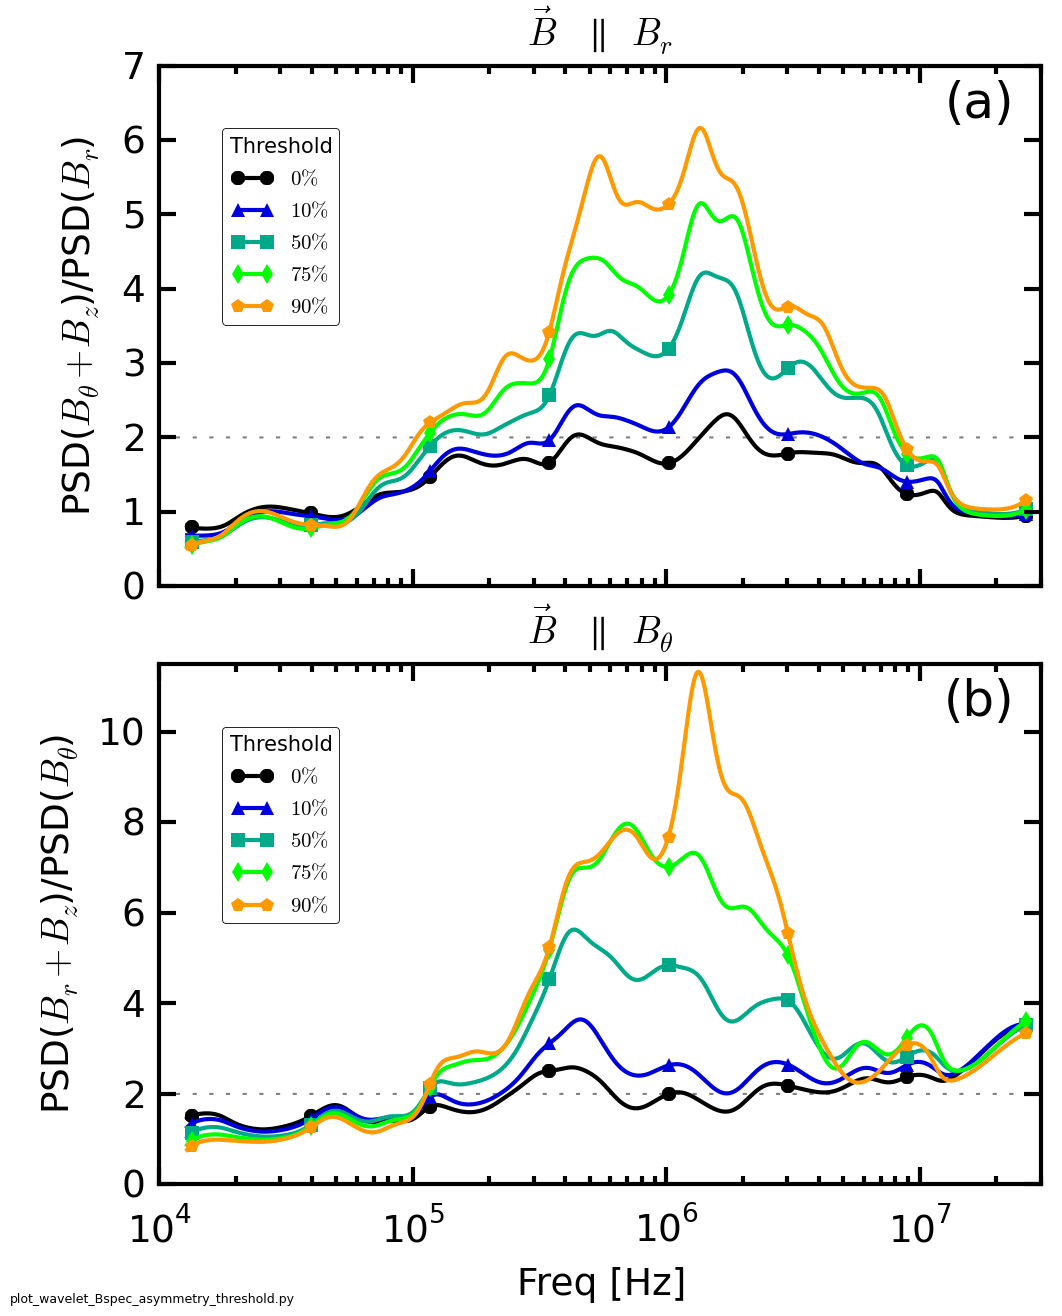
\includegraphics[width=8.5cm]{Bperppara_spectra_thresholdscan40t60us}}
\caption{\label{fig:thresholdmethod}}
\end{figure}

Indeed, an effect like this is observed. Figure~\ref{fig:thresholdmethod} shows the ratio of total perpendicular fluctuation power to parallel fluctuation power for $n = r$(a) and $n = \theta$(b). The threshold fraction is indicated by color. The dashed line at 2 represents isotropy---where the sum of 2 perpendicular components is about twice the power of the single parallel component. Clearly, for the lowest threshold value, the ratio remains close to the isotropy line for all frequencies as would be expected. As the threshold value is raised, the ratio from about 10kHz and higher begins to grow. This shows there is variance anisotropy in the plasma. If the plasma were isotropic, a difference between perpendicular and parallel spectra would not be seen. The anisotropy ratio reaches a maximum as the threshold nears 100\%. The drawback to this method, however, is that as the threshold is increased, the number of individual spectra summed is reduced which increases the error of each curve.

\subsection{Projection Method}

An alternative method, and that used to compute the results presented in this manuscript, uses the $\vec{B}$ timeseries data to project spectral power into perpendicular and parallel portions at each timestep. This projection method uses all the available timesteps and shots rather than making a cut like the threshold method. It will be shown later that the two methods give quantitatively similar answers for the amount of variance anisotropy.

The projection method also uses the Wavelet transform to compute B(f,t). However, that than use the $\vec{B}(t)$ as a threshold value, it is used as a reference vector to determine what fraction of the fluctuation power of $B_{r}(f,t)$, $B_{\theta}(f,t)$, and $B_{z}(f,t)$ is perpendicular or parallel to that vector. The parallel component of each $B_{x}(f,t)$ is found by computing the projection,
\begin{equation}
Proj_{u}v = \frac{\vec{v} \cdot \vec{u}}{||\vec{u}||}\vec{u}
\label{eq:projection}
\end{equation}
which shows that the magnitude of the component of $B_{x}$ parallel to $\vec{B}$ is
\begin{equation}
B_{x}^{\parallel} = \frac{B^{2}_{x}}{|\vec{B}|^{2}}.
\label{eq:para_mag}
\end{equation}
Then, the magnitude of the component perpendicular is
\begin{equation}
B_{x}^{\perp} = 1 - \frac{B^{2}_{x}}{|\vec{B}|^{2}}.
\label{eq:perp_mag}
\end{equation}
Using these projection coefficients, each Wavelet transform spectra, $B_{x}(f,t)$ for $x = r,\theta,z$, can be divided into $B_{x}^{\parallel}(f,t)$ and $B_{x}^{\perp}(f,t)$. For each timestep during each shot, the total parallel and perpendicular power is found by summing the respective portions from each orthogonal direction. These summed quantities, $B^{\parallel}(f,t)$ and $B^{\perp}(f,t)$ are what are used in Section~\ref{sec:variance}.

\begin{figure}[!htbp]
\centerline{
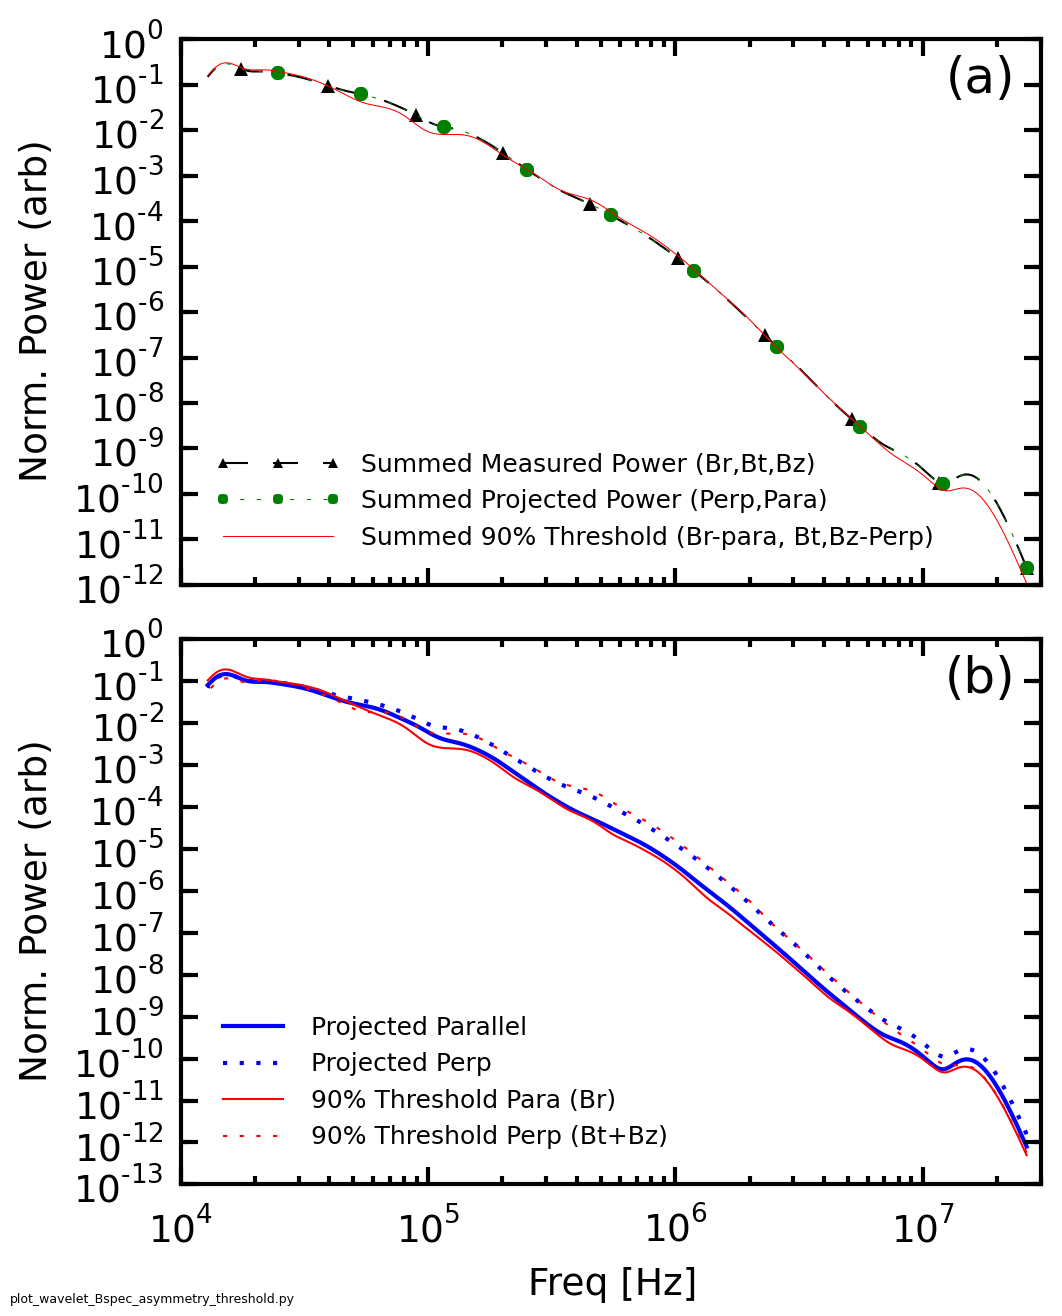
\includegraphics[width=8.5cm]{Bperppara_spectra_thresholdvsprojection40t60us}}
\caption{\label{fig:powercomparison}}
\end{figure}

As a check, the total fluctuation power spectrum is computed in three different ways and plotted in Figure~\ref{fig:powercomparison}(a) for a time range of 40 to 60$\mu s$. The total power is found by (1) summing $B_{r}(f)$, $B_{\theta}(f)$, and $B_{z}$ directly, (2) summing $B^{\parallel}(f)$ and $B^{\perp}(f)$, (3) and summing the 90\% threshold spectra of $B_{r}$, $B_{\theta}$, and $B_{z}$ from the threshold method. The curves are averaged over the total number of timesteps used in their construction so they can be directly compared amongst one another. The first two ways match exactly, showing that the total power is being properly portioned. The 90\% threshold calculation is does not match exactly, though is close. Figure~\ref{fig:powercomparison}(b) shows a comparison of the variance anistropy of the frequency power spectra as computed by the threshold and the projection methods. Again, the curves are normalized to total number of timesteps used in construction. The quantitative comparison shows that the projection method works well to compute the level of anisotropy as it compares well to the more direct, robust threshold method.

\subsection{Local vs. Global Magnetic Field}

\begin{figure}[!htbp]
\centerline{
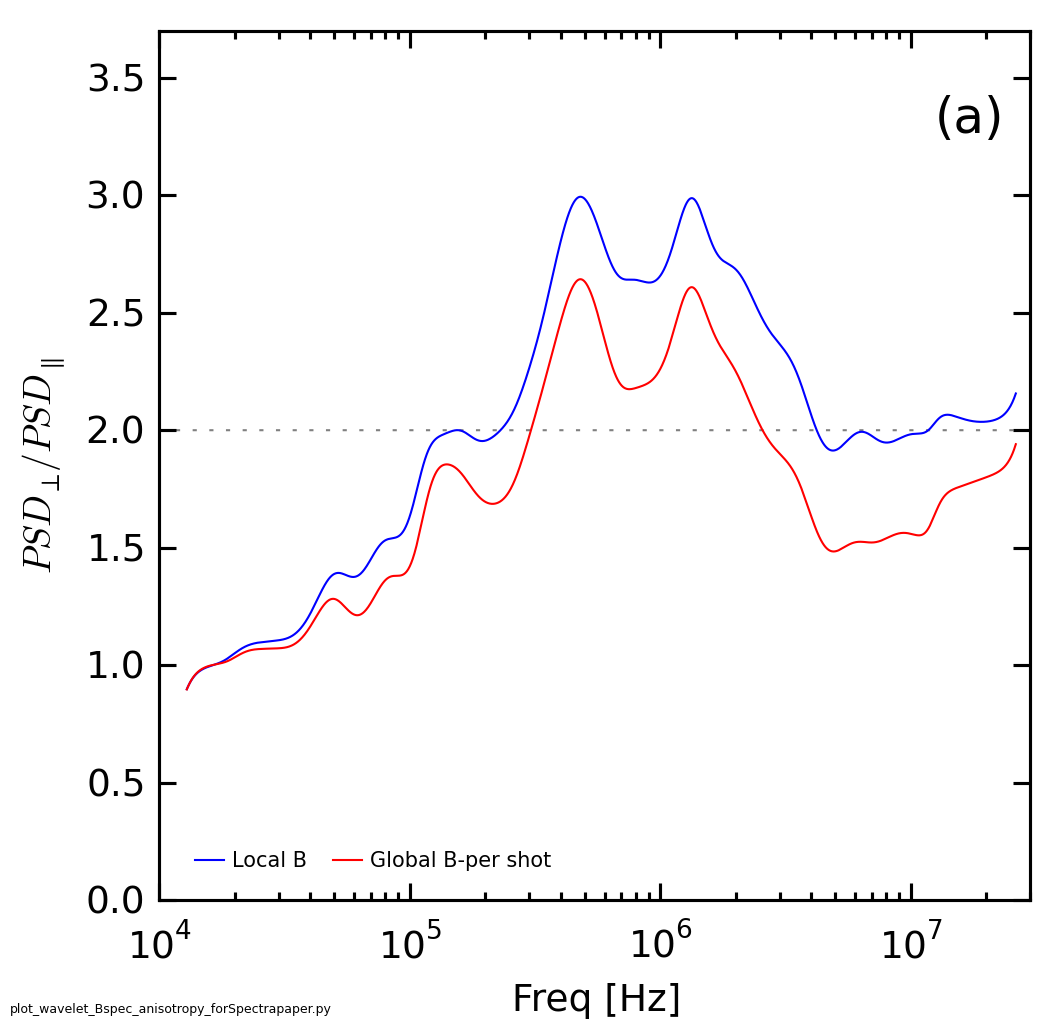
\includegraphics[width=8.5cm]{BperpparaGlobalBcomp_chan1t4_1mWbspectra}}
\caption{\label{fig:globalcomparison}}
\end{figure}

The use of a temporally local versus global magnetic field in anisotropy analysis in the solar wind has been often debated~\cite{podesta09,matthaeus12}. In this paper, a local magnetic field reference vector has been used, but a relative global field can also be used to establish anisotropy. Since the experimental data is extracted on a shot-by-shot basis, the global field in this case is the mean field for the time duration of each shot. Figure~\ref{fig:globalcomparison} shows the anisotropy ratio for local field (reference vector at each timestep) and global field (mean field for each shot). While the local field yields a ratio that is slightly higher than for the global, the trend as a function of frequency is clearly similar. This suggests that though the use of a global versus local field may modify the exact numerical relationship, an anisotropy trend can be observed in either case if it is present in the plasma.
% ----------------------------------------------------------------
\section*{Acknowledgements}
%  We gratefully acknowledge many useful discussions with William Matthaeus. This work has been funded by the US DoE Experimental Plasma Research program and the National Science Foundation.  The simulations were performed using the advanced computing resources (Cray XC30 Edison system) at the National Energy Research Scientific Computing Center.
% ----------------------------------------------------------------
\section*{References}
\begin{thebibliography}{99}

\bibitem{horbury12} T.S. Horbury, R.T. Wicks, C.H.K. Chen. Anisotropy in Space Plasma Turbulence: Solar Wind Observations. Space Sci Rev. {\bf 172} 325-342 (2012).

\bibitem{howes12a} G.G. Howes, D.J. Drake, K.D. Nielson, T.A. Carter, C.A. Kletzing and F. Skiff. Toward Astrophysical Turbulence in the Laboratory. Phys. Rev. Lett. {\bf 109} 255001 (2012).

\bibitem{ren11} Y. Ren, A.F. Almagri, G. Fiksel, S.C. Prager, J.S. Sarff and P.W. Terry. Experimental Observation of Anisotropic Magnetic Turbulence in a Reversed Field Pinch Plasma. Phys. Rev. Lett. {\bf 107} 195002 (2011).

\bibitem{schaffner14a} D.A. Schaffner {\it et al.} Turbulence analysis of an experimental flux rope plasma. {\bf 56} 064003 (2014).

\bibitem{schaffner14b} D.A. Schaffner {\it et al.} Observation of turbulent intermittency scaling with magnetic helicity in an MHD plasma wind-tunnel. Submitted to PRL? Feb 2014.

\bibitem{clauset09}A. Clauset, C. Rohilla Shalizi, M.E.J. Newman, Power-law distributions in empirical data, SIAM Rev. {\bf 51}, 661703 (2009).

\bibitem{roberts10}D. Aaron Roberts. Evolution of the spectrum of solar wind velocity fluctuations from 0.3 to 5 AU. JGR. {\bf 115}, A12 (2010).

\bibitem{podesta09}J.J. Podesta. Dependence of Solar-Wind Power Spectra on the Direction of the Local Mean Magnetic Field. ApJ. {\bf 698}, 986-999 (2009).

\bibitem{matthaeus12}W.H. Matthaeus, S. Servidio, P. Dmitruk, V. Carbone, S. Oughton, M. Wan and K.T. Osman. Local Anisotropy, Higher Order Statistics and Turbulence Spectra. ApJ. {\bf 750}, 103 (2012).

%\bibitem{Belmabrouk98} Belmabrouk, H., and M. Michard (1998), Taylor length scale measurement by laser Doppler velocimetry, Exp. Fluids, 25, 69Ð76.

%\bibitem{Matthaeus05} Matthaeus, W. H. and Dasso, S. and Weygand, J. M. and Milano, L. J. and Smith, C. W. and Kivelson, M. G., Phys. Rev. Lett. 95, 231101 (2005) Spatial Correlation of Solar-Wind Turbulence from Two-Point Measurements

%\bibitem{Weygand07} Weygand, J. M., Matthaeus, W. H., Dasso, S., Kivelson, M. G., and Walker, R. J. (2007), J. Geophys. Res., 112, A10201.

%\bibitem{Weygand09} Weygand, J. M., Matthaeus, W. H., Dasso, S., Kivelson, M. G., Kristler, L. M., and Mouikis, C. (2009), J. Geophys. Res., 114, A07213.

%\bibitem{Weygand10} Weygand, J. M., Matthaeus, W. H., El-Alaoui, M., Dasso, S., and Kivelson, M. G. (2010), J. Geophys. Res., textit115, A12250.

%\bibitem{Weygand11} Weygand, J. M., Matthaeus, W. H., Dasso, S., and Kivelson, M.G. (2011), J. Geophys. Res., 116, A08120.

%\bibitem{Matthaeus08} Matthaeus W. H., Weygand, J. M., Chuychai, P., Dasso, S., Smith, C. W., and Kivelson, M. (2008), Astrophys. J., 678, L141.

%\bibitem{frisch95}Frisch, U. 1995, {\it Turbulence} (Cambridge: Cambridge Univ. Press)

%\bibitem{sorrisovalvo99}Sorriso-Valvo, L. {\it et al.} Geophys. Res. Lett. {\bf 26}, 1801–1804 (1999).

%\bibitem{wan12}Wan, M. {\it et al.} ApJ. {\bf 744} 177 (2012).

%\bibitem{sorrisovalvo01}Sorriso-Valvo, L. {\it et al.} Planet. Space Sci. {\bf 49}, 1193–1200 (2001).

%\bibitem{marrelli05}Marrelli, L. {\it et al.} Phys. Plasmas. {\bf 12}, 030701 (2005).

%\bibitem{Greco08}A. Greco, P. Chuychai, W. H. Matthaeus, S. Servidio and P. Dmitruk, Intermittent MHD structures and classical discontinuities, Geophys. Res. Lett. {\bf 35}, L19111 (2008).

%\bibitem{Greco09}Greco, A., Matthaeus, W. H., Servidio, S., Chuychai, P., and Dmitruk, P.: Statistical Analysis of Discontinuities in Solar Wind ACE Data and Comparison with Intermittent MHD Turbulence, ApJ {\bf 691}, L111 (2009).

%\bibitem{Wan09}Wan, M., Oughton, S., Servidio, S., and Matthaeus, W. H.: Generation of non-Gaussian statistics and coherent structures in ideal magnetohydrodynamics, Phys. Plasmas {\bf 16}, 080703 (2009).

%\bibitem{Servidio11b}Servidio, S. {\it et al}, J. Geophys. Res. {\bf 116}, A09102 (2011).

%\bibitem{Gray13} T. Gray, M. R. Brown, and D. Dandurand. Phys. Rev. Lett. {\bf 110}, 085002 (2013). 



%\bibitem{Taylor86} J. B. Taylor, Rev. Mod. Phys. {\bf 58}, 741 (1986).

%\bibitem{Matthaeus80} W.H. Matthaeus and D. Montgomery, Ann. N.Y. Acad. Sci. {\bf 357}, 203 (1980).

%\bibitem{torrence98}C. Torrence, G.P. Compo, A practical guide to wavelet analysis. Bull. Am. Meteorol. Soc. {\bf 79}, 6178 (1998).



%\bibitem{wan12}M. Wan, K. T. Osman, W. H. Matthaeus, and S. Oughton, Investigation of intermittency in magnetohydrodynamics and solar wind turbulence: scale-dependent kurtosis, ApJ {\bf 744}, 171 (2012).

%\bibitem{Gray10}T. Gray, V. S. Lukin, M. R. Brown, C. D. Cothran, Three-dimensional reconnection and relaxation of merging spheromak plasmas, Phys. Plasmas {\bf 17}, 102106 (2010).

%\bibitem{goldstein94}Goldstein, M.L., Roberts, D.A. and Fitch, C.A. Jour. Geo. Res. {\bf 99} 11519-11538 (1994).

%\bibitem{ji95}Ji, H., Prager, S.C. and Sarff, J.S. Phys. Rev. Lett. {\bf 74} 2945 (1995).

%\bibitem{telloni12}Telloini, D. {\it et al.}. ApJ. {\bf 751} 19 (2012).

%\bibitem{matthaeusVelli11}Matthaeus, W.H. and Velli, M. Space Sci. Rev. {\bf 160} 145-168 (2011).

%\bibitem{greco12}A. Greco {\it et al.} ApJ. {\bf 749} 105 (2012).

\end{thebibliography}

\end{document}

